\documentclass[
	%parspace, % Add vertical space between paragraphs
	%noindent, % No indentation of first lines in each paragraph
	%nohyp, % No hyphenation of words
	%twoside, % Double sided format
	%draft, % Quicker draft compilation without rendering images
	%final, % Set final to hide todos
]{elteikthesis}[2022/04/30]
\usepackage{epigraph}
\usepackage{enumitem}
\usepackage{setspace}

% The minted package is also supported for source highlighting
% See minted-intregration.tex for example
\usepackage[newfloat]{minted}
% \usepackage{setspace}

% Document's metadata
\title{Static security code analysis using LLVM compiler frontend} % title
\date{2022} % year of defense

% Author's metadata
\author{Cristea Andrei}
\degree{Computer Science BSc}

% Superivsor(s)' metadata
\supervisor{ Gera Zoltan} % internal supervisor's name
\affiliation{Assistant Professor, PhD} % internal supervisor's affiliation
%\extsupervisor{Jane Doe} % external supervisor's name
%\extaffiliation{Senior Developer} % external supervisor's affiliation

% University's metadata
\university{Eötvös Loránd University} % university's name
\faculty{ Faculty of Informatics} % faculty's name
\department{\small Department of Programming Languages and Compilers } % department's name
\city{Budapest} % city
\logo{elte_cimer_szines} % logo

% Add bibliography file
\addbibresource{elteikthesis.bib}

% The document
\begin{document}

% Set document language
%\documentlang{hungarian}
\documentlang{english}

% Title page (mandatory)
\maketitle

% Topic declaration page (mandatory) - can also be attached instead
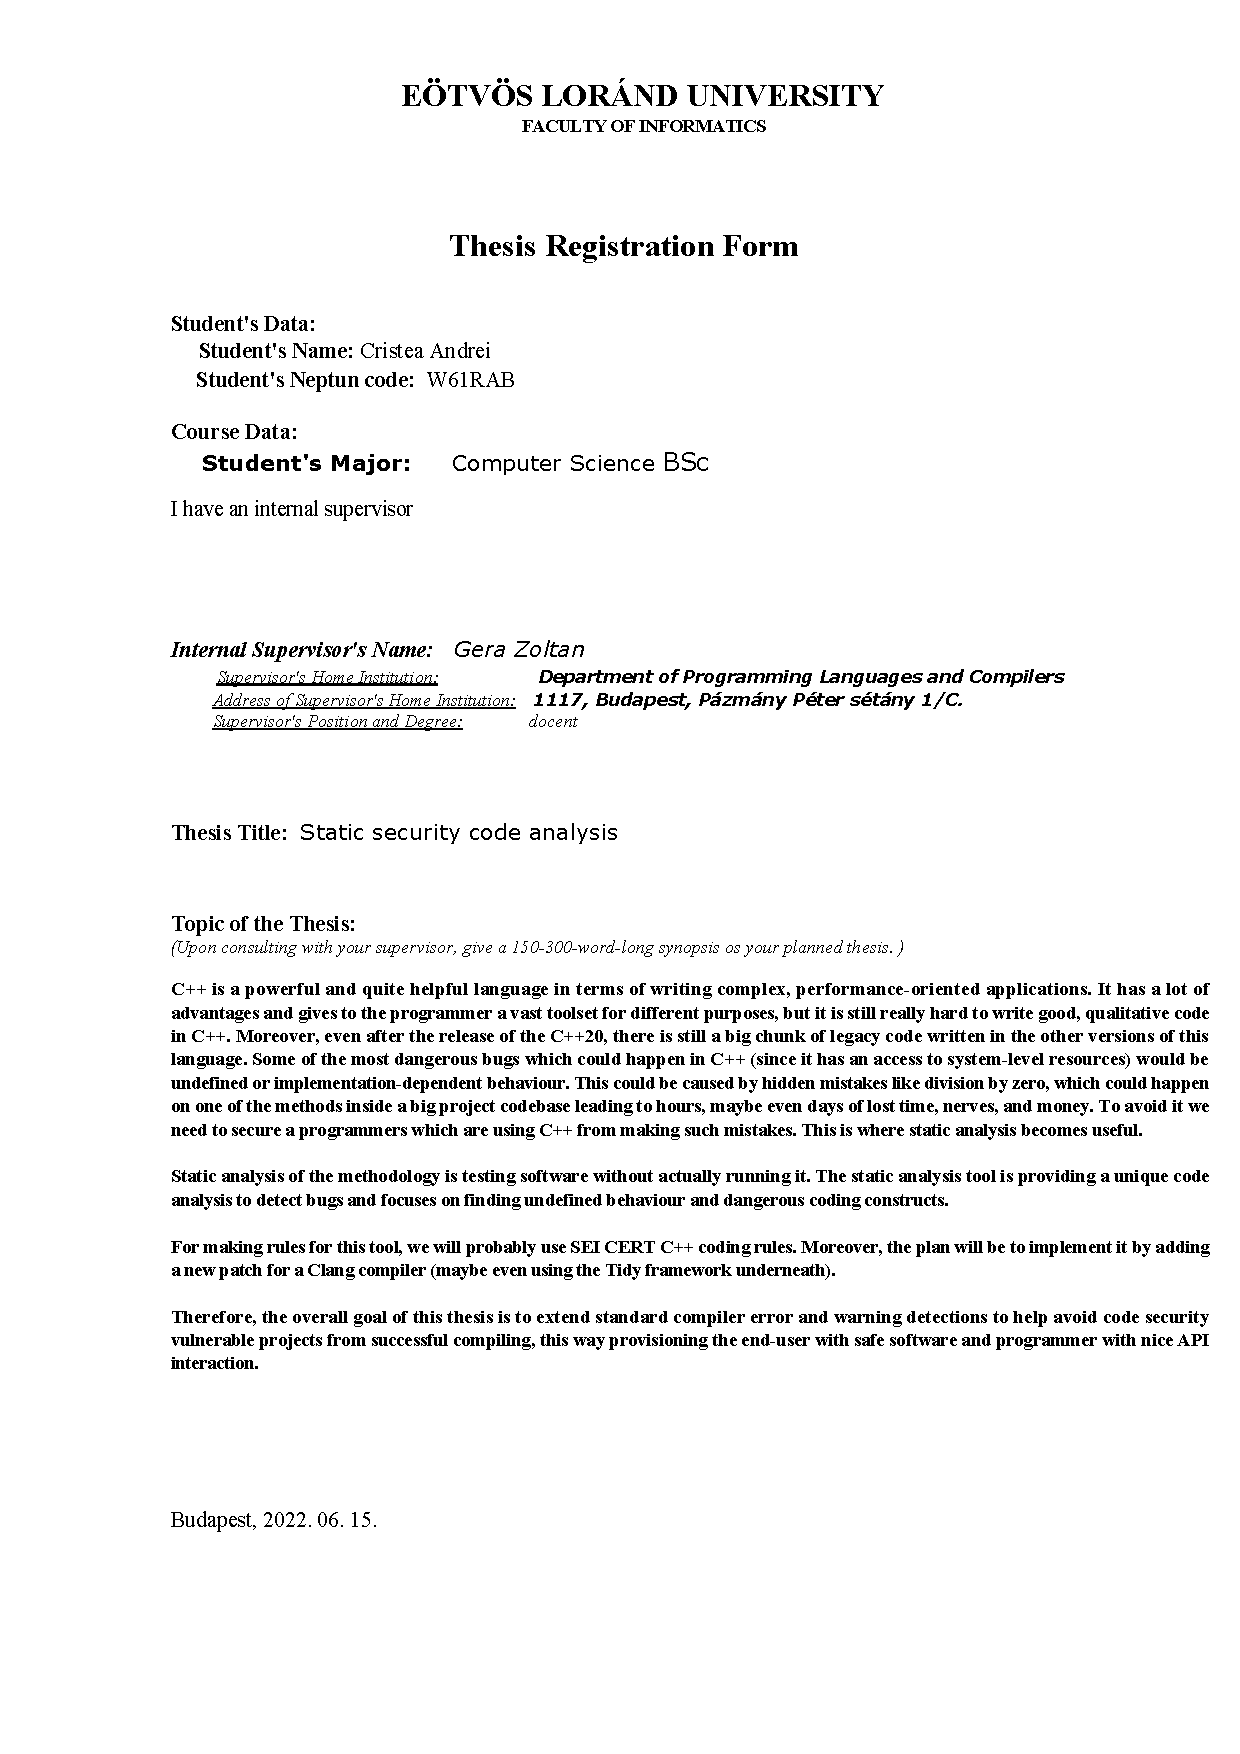
\includepdf{topicdeclaration.pdf}

% Table of contents (mandatory)
\tableofcontents
\cleardoublepage

% Structure
\chapter{Summary}

The closer we come to human technological advancement, the more people start to get involved in this splendid world of programming. At the same time, we live in the Renaissance of programming languages. The importance of static analysis tools is to use correctly the programming languages, according to the guidelines and standards, to make it more professional. This thesis aimed to the part of this community effort.


It presented an overview of LLVM and clang-tidy in particular, and a solution for static analysis check of a particular set of bugs in C/C++ which are caused by unexpected behavior of the program. The thesis concentrated on explaining to the reader the basic examples of the consequences of violating those warnings, and a short guideline into Clang AST and marcher creation pipeline.  In the course of the development, two possible solutions for the matcher were found, and both of those were tested and checked through the categories in order to find the best match for the community code. 

Even though the top-down matcher was chosen in the end, the important lessons were taken from the bottom-up solution as well. There is still a big field of performance testing and adjustments which can make the checker work faster, which has a big importance for the IDE in particular. Moreover, a vast field of code readability and its implementations was found, which has a lot of good theory material has not so many practice references.

Altogether, it was a great experience working in the compiler front-end field, both as getting practice knowledge and theory application, plus contributing to the largest codebase in the world. Therefore, it is a great study material for the demonstration of the knowledge and experience achieved through my bachelor studies, and my personal triumph over one more field of computer science, and life in general.  
\cleardoublepage
\chapter{Summary}

The closer we come to human technological advancement, the more people start to get involved in this splendid world of programming. At the same time, we live in the Renaissance of programming languages. The importance of static analysis tools is to use correctly the programming languages, according to the guidelines and standards, to make it more professional. This thesis aimed to the part of this community effort.


It presented an overview of LLVM and clang-tidy in particular, and a solution for static analysis check of a particular set of bugs in C/C++ which are caused by unexpected behavior of the program. The thesis concentrated on explaining to the reader the basic examples of the consequences of violating those warnings, and a short guideline into Clang AST and marcher creation pipeline.  In the course of the development, two possible solutions for the matcher were found, and both of those were tested and checked through the categories in order to find the best match for the community code. 

Even though the top-down matcher was chosen in the end, the important lessons were taken from the bottom-up solution as well. There is still a big field of performance testing and adjustments which can make the checker work faster, which has a big importance for the IDE in particular. Moreover, a vast field of code readability and its implementations was found, which has a lot of good theory material has not so many practice references.

Altogether, it was a great experience working in the compiler front-end field, both as getting practice knowledge and theory application, plus contributing to the largest codebase in the world. Therefore, it is a great study material for the demonstration of the knowledge and experience achieved through my bachelor studies, and my personal triumph over one more field of computer science, and life in general.  
\cleardoublepage
\chapter{Summary}

The closer we come to human technological advancement, the more people start to get involved in this splendid world of programming. At the same time, we live in the Renaissance of programming languages. The importance of static analysis tools is to use correctly the programming languages, according to the guidelines and standards, to make it more professional. This thesis aimed to the part of this community effort.


It presented an overview of LLVM and clang-tidy in particular, and a solution for static analysis check of a particular set of bugs in C/C++ which are caused by unexpected behavior of the program. The thesis concentrated on explaining to the reader the basic examples of the consequences of violating those warnings, and a short guideline into Clang AST and marcher creation pipeline.  In the course of the development, two possible solutions for the matcher were found, and both of those were tested and checked through the categories in order to find the best match for the community code. 

Even though the top-down matcher was chosen in the end, the important lessons were taken from the bottom-up solution as well. There is still a big field of performance testing and adjustments which can make the checker work faster, which has a big importance for the IDE in particular. Moreover, a vast field of code readability and its implementations was found, which has a lot of good theory material has not so many practice references.

Altogether, it was a great experience working in the compiler front-end field, both as getting practice knowledge and theory application, plus contributing to the largest codebase in the world. Therefore, it is a great study material for the demonstration of the knowledge and experience achieved through my bachelor studies, and my personal triumph over one more field of computer science, and life in general.  
\cleardoublepage
\chapter{Summary}

The closer we come to human technological advancement, the more people start to get involved in this splendid world of programming. At the same time, we live in the Renaissance of programming languages. The importance of static analysis tools is to use correctly the programming languages, according to the guidelines and standards, to make it more professional. This thesis aimed to the part of this community effort.


It presented an overview of LLVM and clang-tidy in particular, and a solution for static analysis check of a particular set of bugs in C/C++ which are caused by unexpected behavior of the program. The thesis concentrated on explaining to the reader the basic examples of the consequences of violating those warnings, and a short guideline into Clang AST and marcher creation pipeline.  In the course of the development, two possible solutions for the matcher were found, and both of those were tested and checked through the categories in order to find the best match for the community code. 

Even though the top-down matcher was chosen in the end, the important lessons were taken from the bottom-up solution as well. There is still a big field of performance testing and adjustments which can make the checker work faster, which has a big importance for the IDE in particular. Moreover, a vast field of code readability and its implementations was found, which has a lot of good theory material has not so many practice references.

Altogether, it was a great experience working in the compiler front-end field, both as getting practice knowledge and theory application, plus contributing to the largest codebase in the world. Therefore, it is a great study material for the demonstration of the knowledge and experience achieved through my bachelor studies, and my personal triumph over one more field of computer science, and life in general.  
\cleardoublepage

% Acknowledgements (optional) - in case your thesis received funding or would like to express special thanks to someone
\chapter*{\acklabel}
\addcontentsline{toc}{chapter}{\acklabel}

I would like to thank the people, who were the most helpful throughout the whole thesis preparation, with whom I could grow as a person and student, and without whom I can not see myself being an undergraduate student. 

Firstly, I would like to thank my supervisor, Prof. Zoltán Gera, for his suggestion of the thesis topic, for helping to understand the framework I used for this thesis, and for guiding me through each step of the work, with the suggestions and critique. Prof. Zoltán has ready to guide me every week if I had any complications and explained how to use LLVM documentation. Overall, it was a great pleasure to be under his supervision, and work in the team with others implementors of the clang-tidy checks.   

I also would like to give big gratitude to my compilers professor Horpacsi Daniel, who gave me great insights about how the compilers work, parsing techniques in particular. With his help, I could understand such concepts as LL, and LR parsing and its limitations. Plus, Prof. Horpacsi Daniel also gave me consultations when I was stuck with my implementation, and provided some insights about how I can extend my work.  

I am also grateful for the other professors of ELTE who were not mentioned above, all of them made great work in improving my skills for becoming a better developer and Computer Science student. 

% % Appendices (optional) - useful for detailed information in long tables, many and/or large figures, etc.
\appendix
\chapter{List of created and modified files} % Simulation results
\label{appx:files}

Changes were made only in \lstinline{llvm-project/clang-tools-extra} directory.


\section{List of modified files for EXP45-C}

\begin{itemize}
    \item clang-tools-extra/docs/clang-tidy/checks/list.rst
    \item clang-tools-extra/docs/ReleaseNotes.rst
    \item clang-tools-extra/clang-tidy/cert/CERTTidyModule.cpp
    \item clang-tools-extra/clang-tidy/cert/CMakeLists.txt
\end{itemize}

\section{List of added files for EXP45-C}

\begin{itemize}
    \item clang-tools-extra/docs/clang-tidy/checks/cert-assignments-in-selection.rst
    \item clang-tools-extra/clang-tidy/cert/AssignmentsInSelectionCheck.cpp
    \item clang-tools-extra/clang-tidy/cert/AssignmentsInSelectionCheck.h
    \item clang-tools-extra/test/clang-tidy/checkers/cert-assignments-in-selection.cpp
\end{itemize}
\cleardoublepage

% % Bibliography (mandatory)
\phantomsection
\addcontentsline{toc}{chapter}{\biblabel}
\printbibliography[title=\biblabel]
\cleardoublepage

% % List of figures (optional) - useful over 3-5 figures
\phantomsection
\addcontentsline{toc}{chapter}{\lstfigurelabel}
\listoffigures
\cleardoublepage

% % List of tables (optional) - useful over 3-5 tables
\phantomsection
\addcontentsline{toc}{chapter}{\lsttablelabel}
\listoftables
\cleardoublepage

% % List of codes (optional) - useful over 3-5 code samples
\phantomsection
\addcontentsline{toc}{chapter}{\lstcodelabel}
\lstlistoflistings
\cleardoublepage

% List of symbols (optional)
%\printnomenclature

\end{document}
